\section{Background}
This document is a recapitulation of a discussion regarding a proposal of future scenarios by ChildFund Alliance. The aim of that proposal being to provide add-ons, new elements as well as alternatives to the current sponsorship model.

This document is also to provide suggestions for possible extensions to the ChildFund Alliance (CFA) proposal which can add value as well as potentially deepen the understanding of opportunity in the proposal.

Each section of this document is based around a chapter or rather a "gear" from the book – \textbf{Gear Up your best business idea ever}. This is to serve as both a way for the students to familiarize themselves with the concepts and values of the book but also learn how to apply them by using the CFA proposal as a case.

\section{What are the pains of the customer?} % (fold)
\label{sec:what_are_the_pains_of_the_customer_}
This section lists the customer pains that were discussed around the CFA proposal. With customer pain we refer not to the physical pain but rather the frustrations and limitations that we as consumers find in everyday life. By being able to identify these specific pains, one drastically increases the chances of being able to "kill" those pains and subsequently create a great product. So, in order to understand the customer we need to understand their pain.

Whether your selling a physical product or offering a service the bottom line is the same: if you interact with your potential customers directly, that is \textbf{not} by using information gathered from computers but actually interacting with them, you will be able to observe and understand their pain.

What's more important is to understand that this is an ongoing process, it never ends. During our discussions in class we made parallels with great entrepreneurs and visionaries like Steve Jobs (Apple) and Henry John Heinz (Heinz), who are known for their tenacity and seemingly endless supply of energy that they put into their products to improve and innovate. Steve Jobs was known to pop in to Apple stores and talk to customers on the products that Apple was offering.

When discussing the proposal during a workshop the class attempted to identify some of the more prominent pains and explain what and why these exist.

\blankpage

\subsection{Looking at current sponsors' pain} % (fold)
\label{sub:looking_at_current_sponsors_pain}

The pain of the current sponsors seems to be that they have none or very limited ways of interacting with the people that they sponsor. 

\begin{quote}
"They didn't have a quick way of getting feedback from the people that are sponsoring. It appears that they way the it works now is that it takes around three months before the sponsor receives updates or feedback. Apparently, there is currently no immediate way for the sponsors and the receivers of the sponsorship to actually connect in a more direct manner. As a solution the CFA made the "Sponsorship Steam" concept."
\end{quote}

To deal with this pain the CFA are suggesting to develop a social platform where the sponsors can receive more immediate feedback as well as interact with other sponsors and CFA itself. However, upon some discussion of the concept "Sponsorship Stream" it became apparent that the CFA's views of how we interact on social media is not based on observation but rather speculation.

% subsection looking_at_current_sponsors (end)

\subsection{Misconception on the use of social media} % (fold)
\label{sub:misconception_on_the_use_of_social_media}

Even though the "Sponsorship Stream" concept might solve the issue of direct feedback the class was unsure of how it would be accepted by customers.

\begin{quote}
"It would seem that the CFA didn't keep up with changes in social media. This in turn shows a gap of how we act on social media now and how they think we act."
\end{quote}

The group explored the notion of having something like a "Sponsorship Stream" in their feed and quickly dismissed it on the basis that it wouldn't provide them with any added value.

We live in a kind of over-communicated and over-informed age where most of the information that is shared is superfluous and most of the time irrelevant. In some cases we would also argue that the main message is sometimes lost.

We urge the CFA to investigate this further but also to tie in potential users and explore the concept to see whether the results are desirable.

% subsection misconception_on_the_use_of_social_media (end)

As the discussion carried on we also had to delve into who the CFA customer is. 

% section what_are_the_pains_of_the_customer_ (end)

\blankpage

\section{Who is the customer?} % (fold)
\label{sec:who_is_the_customer_}

Simply put, a customer is the person who is willing to pay to use your product. In this case, it was quite apparent who the customer was – the sponsors. The CFA has also done a fine job at posing arguments for them in general but what seems to be lacking is an overall understanding that different stakeholders in the process require different types of arguments. This in itself is also a challenge and could potentially be made more clear.

As an example, in the "Active Participation" concept the business model puts the customer segment to be more targeted towards companies rather than individuals and is at the same time stating that it aims to "turn passive sponsors into active members".

Lastly, when the class discussed the different concepts we found two issues that needs to be addressed by the CFA:

\begin{enumerate}
  \item Who is your target customer? What are their pains? Is the pain the same? Apply the pain circle!

  \begin{figure}[htbp]
    \centering
      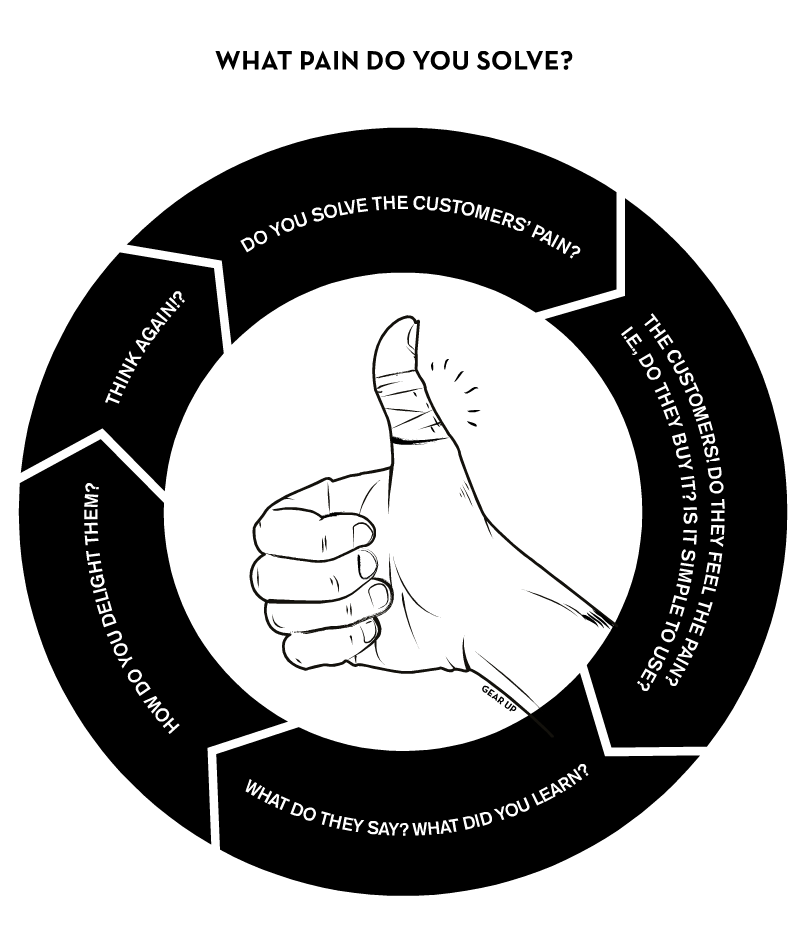
\includegraphics[height=4.5in]{../images/paincircle.png}
    \caption{The Pain Circle – the ongoing process of customer pain \protect\cite{Ramfelt}}
    \label{fig:images_paincircle}
  \end{figure}
  
  \item Although it is refreshing with several concepts it would probably be beneficial if you start with on to two concepts and narrow those down which can then later be built upon.
\end{enumerate}

% section who_is_the_customer_ (end)
